% ------------------------------------------------------------------------------
% TYPO3 CMS 8.5 - What's New - Chapter "Backend User Interface" (Spanish Version)
%
% @author	Michael Schams <schams.net>
% @license	Creative Commons BY-NC-SA 3.0
% @link		http://typo3.org/download/release-notes/whats-new/
% @language	English
% ------------------------------------------------------------------------------
% LTXE-CHAPTER-UID:		07b25346-95b1df21-a6ebe09a-49f53f41
% LTXE-CHAPTER-NAME:	Backend User Interface
% ------------------------------------------------------------------------------

\section{Interfaz de Usuario de Backend}
\begin{frame}[fragile]
	\frametitle{Interfaz de Usuario de Backend}

	\begin{center}\huge{Capítulo 1:}\end{center}
	\begin{center}\huge{\color{typo3darkgrey}\textbf{Interfaz de Usuario de Backend}}\end{center}

\end{frame}

% ------------------------------------------------------------------------------
% LTXE-SLIDE-START
% LTXE-SLIDE-UID:		3c948208-fa0a3ea5-8f3cf70e-6d51607c
% LTXE-SLIDE-ORIGIN:	e00709d6-ccb8a4d0-1cca1d28-431a00a5 English
% LTXE-SLIDE-TITLE:		#77910: New Form Framework (1)
% ------------------------------------------------------------------------------
\begin{frame}[fragile]
	\frametitle{Interfaz de Usuario de Backend}
	\framesubtitle{Nuevo Marco de trabajo para Formulario (1)}

	\begin{itemize}
		\item Se ha integrado un nuevo y flexible framework para construir formularios en TYPO3 CMS 8.5
		\item Reemplaza el \textit{Asistente de Formulario} basado en ExtJS y el sistema de renderizado de frontend dependiente
		\item El nuevo \textit{Editor de Formulario} usa jQuery y usa una arquitectura moderna,
			asegurando alta flexibilidad y extensibilidad
		\item Altamente configurable y los ajustes de configuración son almacenados en ficheros YAML
		\item La lista de características es impresionante\newline
			\small(manténgase al tanto para la documentación al completo)\normalsize
		\item Vídeo de demostración de una preview está disponible en YouTube:\newline
			\url{https://www.youtube.com/watch?v=F9sTAOEcTI0}
	\end{itemize}

\end{frame}
% ------------------------------------------------------------------------------
% LTXE-SLIDE-START
% LTXE-SLIDE-UID:		7200f886-2b4633b9-cee5f782-27206c16
% LTXE-SLIDE-ORIGIN:	3bbca669-629eab1c-0230fd06-71e7071c English
% LTXE-SLIDE-TITLE:		#77910: New Form Framework (2)
% ------------------------------------------------------------------------------
\begin{frame}[fragile]
	\frametitle{Interfaz de Usuario de Backend}
	\framesubtitle{Nuevo Marco de trabajo para Formulario (2)}

	\begin{figure}
		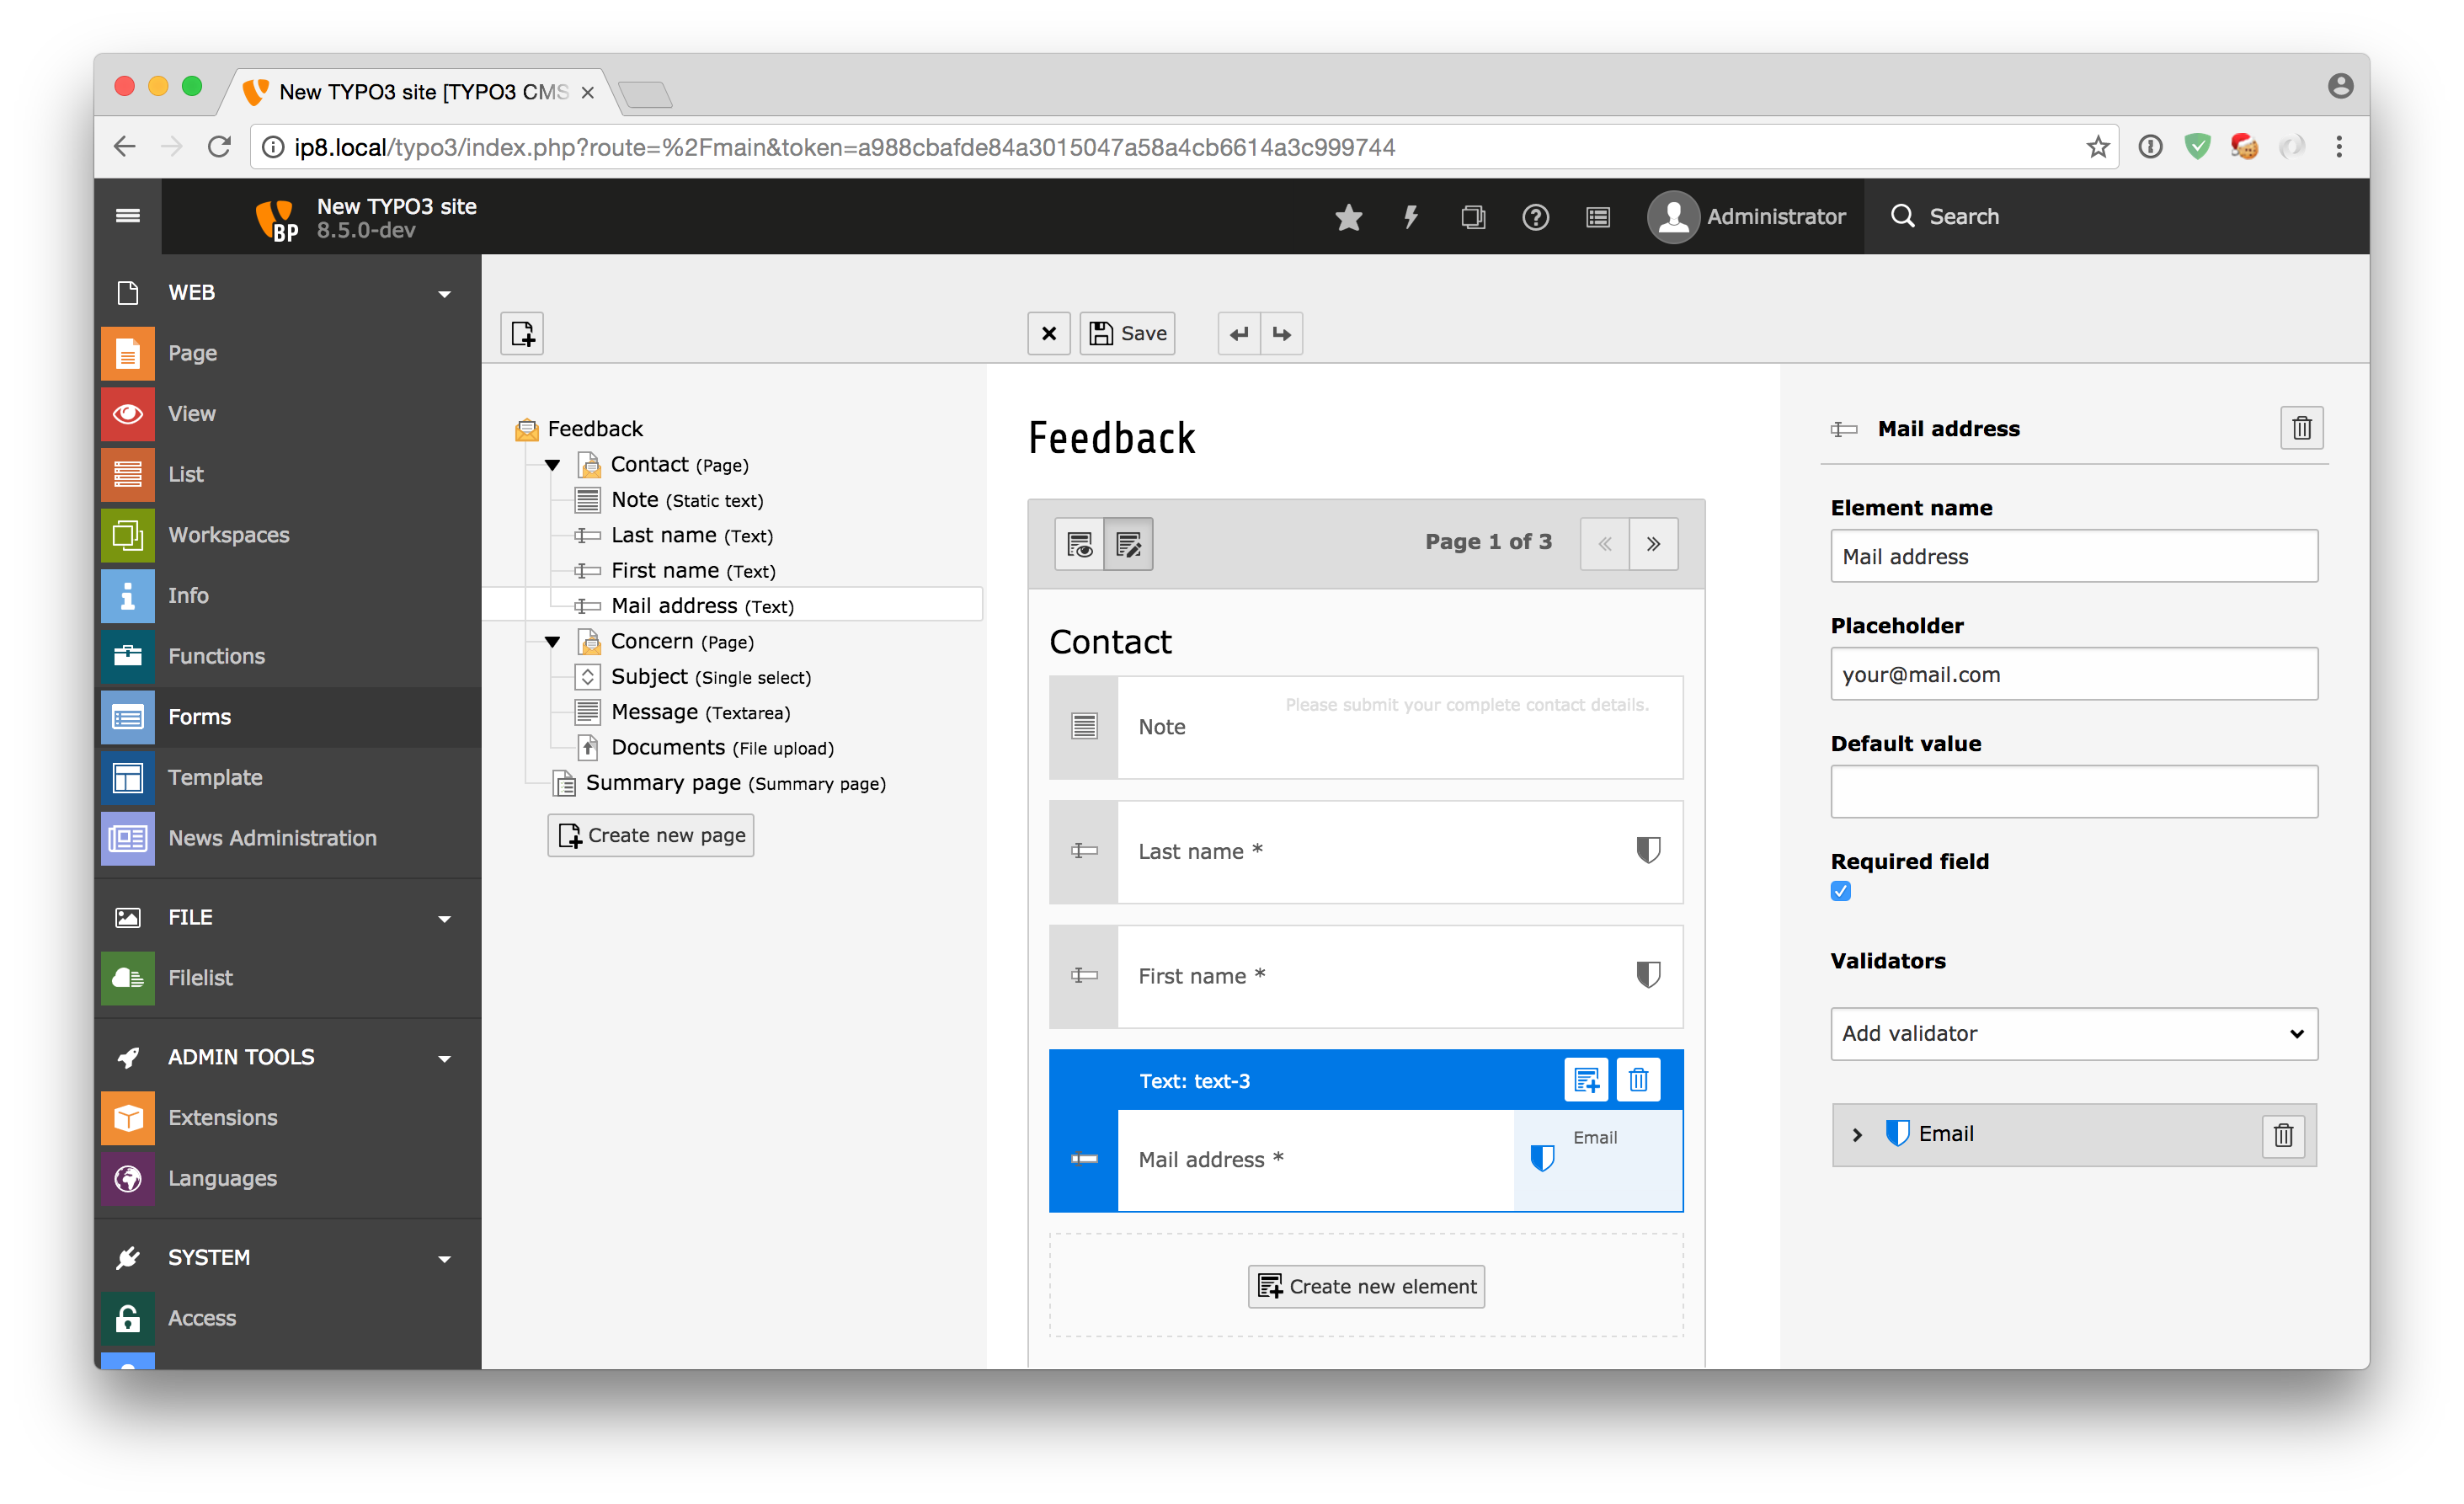
\includegraphics[width=0.8\linewidth]{BackendUserInterface/form-framework-1.png}
	\end{figure}

\end{frame}

% ------------------------------------------------------------------------------
% LTXE-SLIDE-START
% LTXE-SLIDE-UID:		7353f491-9a18706f-6c8c5987-0529435f
% LTXE-SLIDE-ORIGIN:	b91ec75b-7aa7b566-b523ca5f-f9ba3cde English
% LTXE-SLIDE-TITLE:		#77910: New Form Framework (3)
% ------------------------------------------------------------------------------
\begin{frame}[fragile]
	\frametitle{Interfaz de Usuario de Backend}
	\framesubtitle{Nuevo Marco de trabajo para Formulario (3)}

	\begin{figure}
		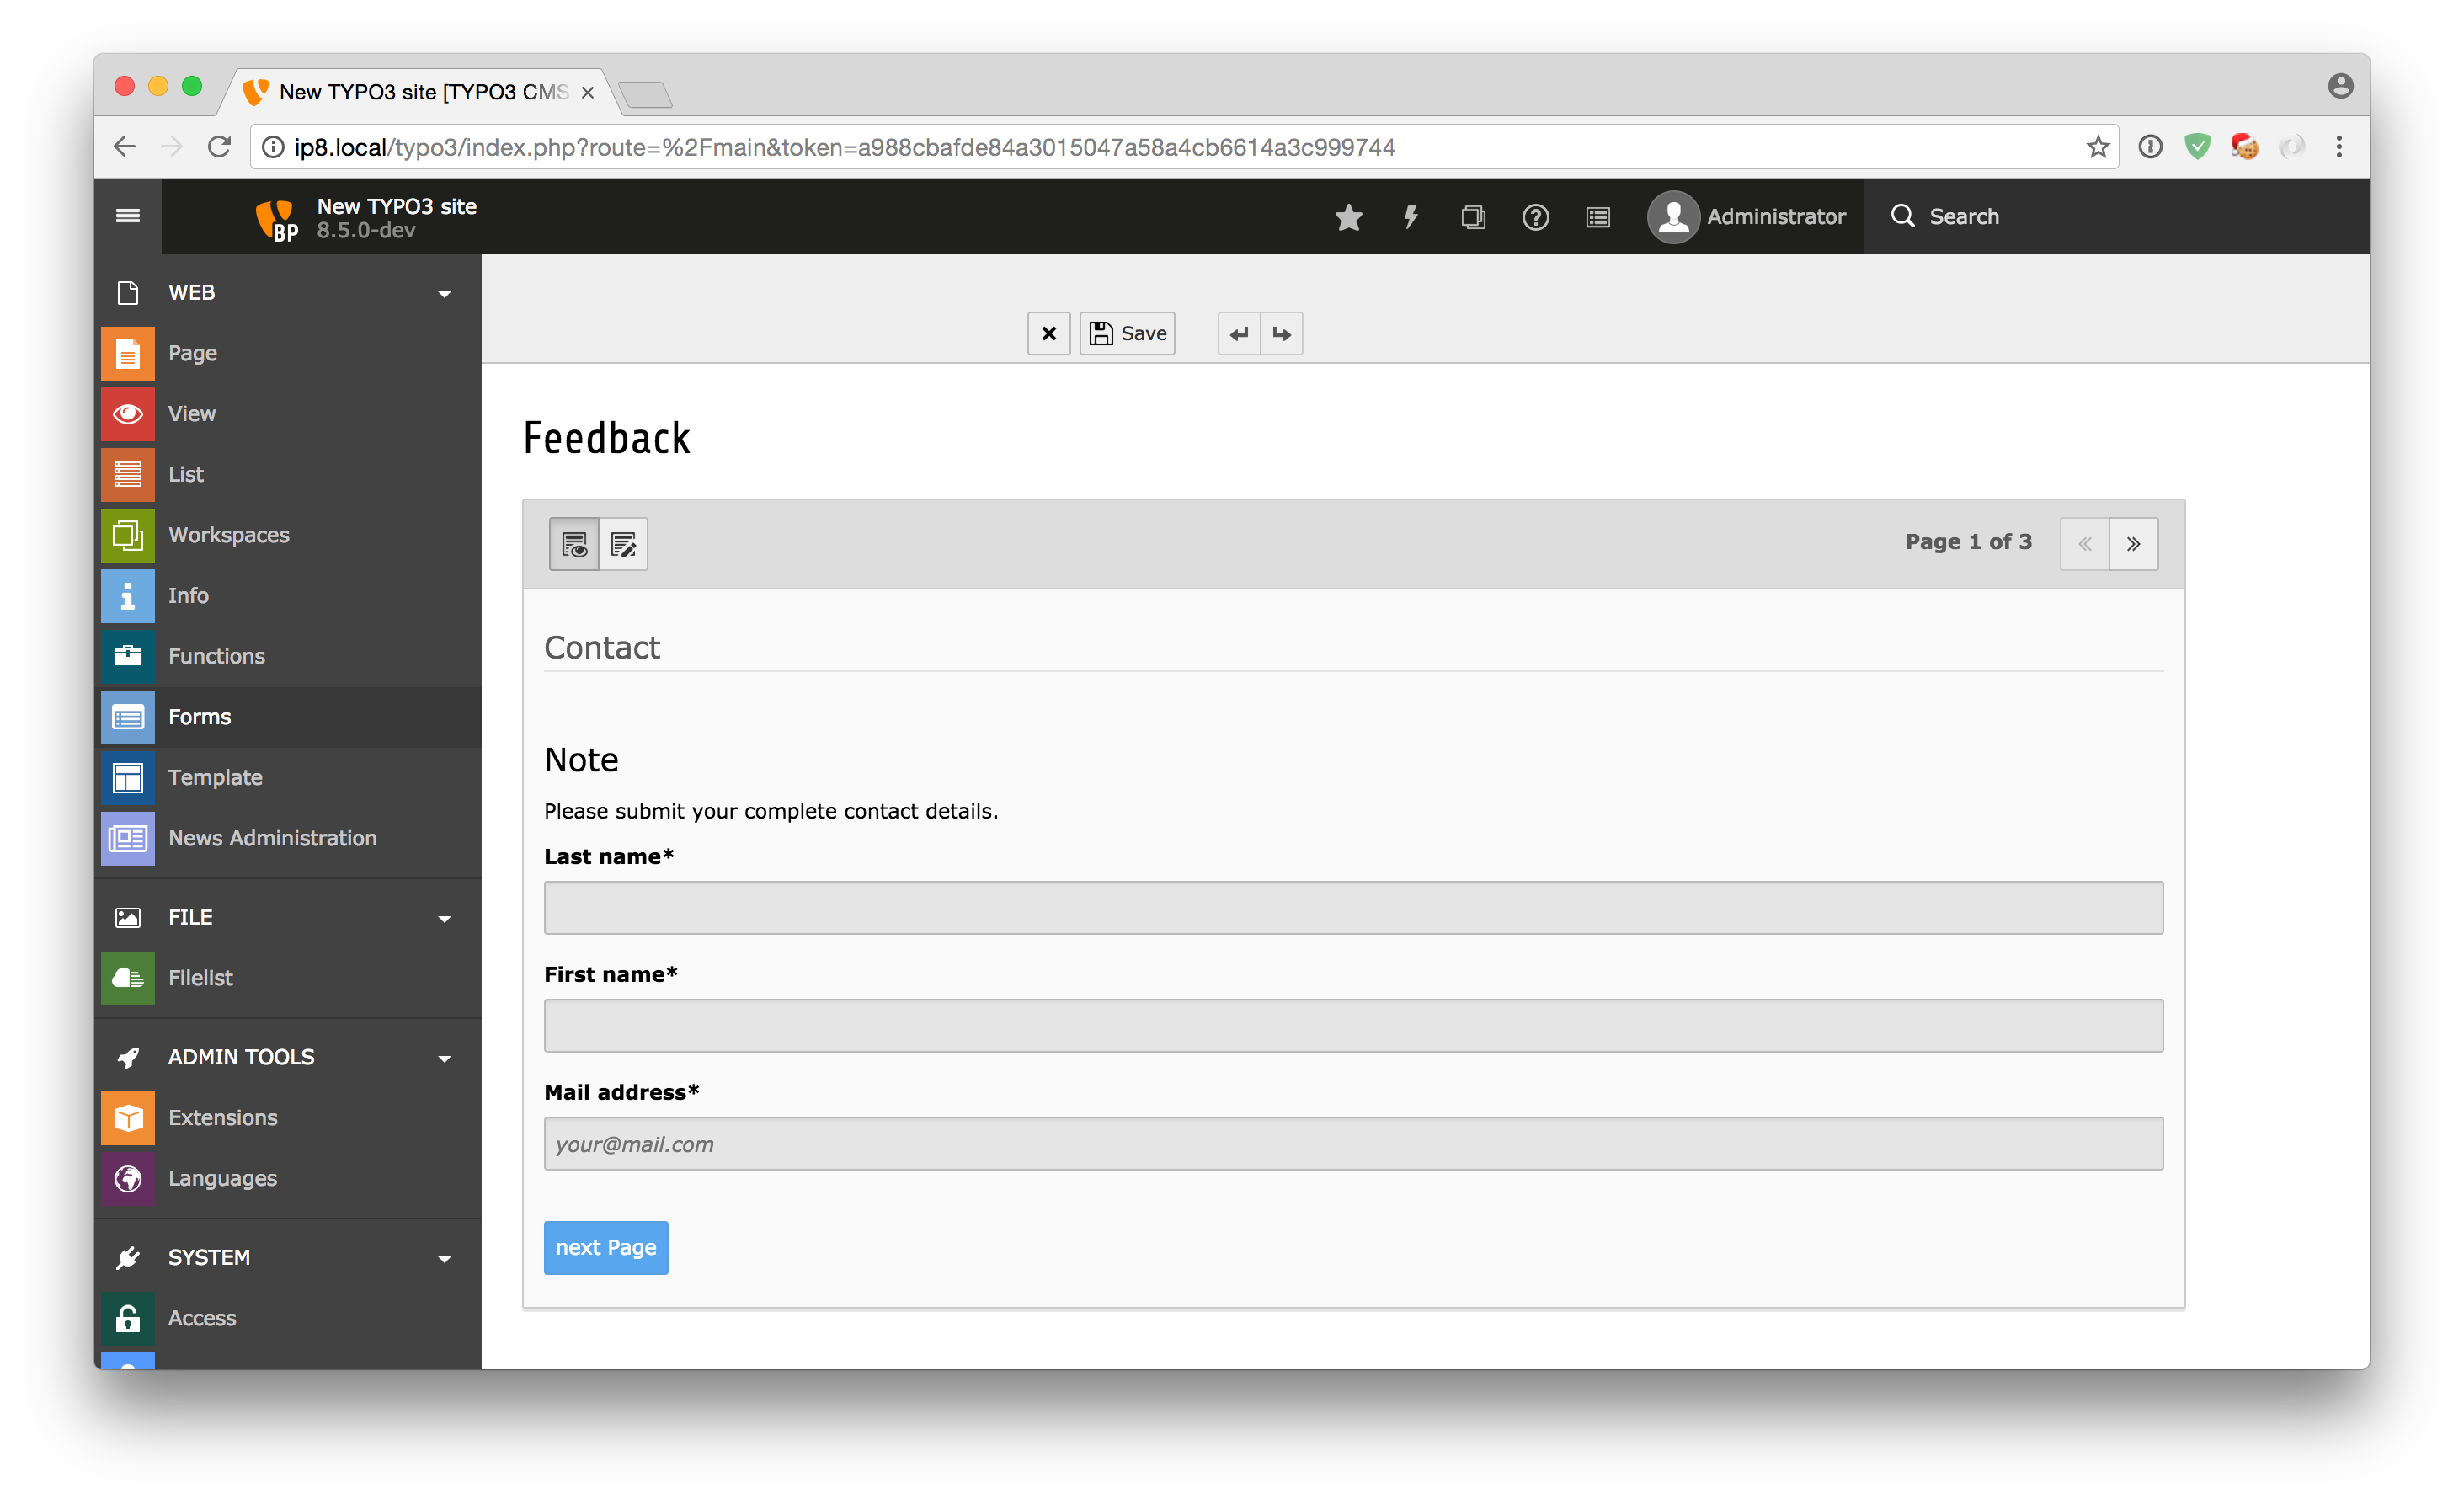
\includegraphics[width=0.8\linewidth]{BackendUserInterface/form-framework-2.png}
	\end{figure}

\end{frame}


% ------------------------------------------------------------------------------
% LTXE-SLIDE-START
% LTXE-SLIDE-UID:		6a41e672-ced4620b-ee3e255c-c9e1faba
% LTXE-SLIDE-ORIGIN:	c41b2f21-fb92bb80-56e7ddc9-1c725e34 English
% LTXE-SLIDE-TITLE:		CKEditor Integration
% ------------------------------------------------------------------------------
\begin{frame}[fragile]
	\frametitle{Interfaz de Usuario de Backend}
	\framesubtitle{Integración de CKEditor (1)}

	\begin{columns}[T]
		\begin{column}{.5\textwidth}
			La siguiente generación de edición de texto enriquecido ha sido implementada en el backend de TYPO3:
			\textbf{CKEditor}.\newline

			El estado actual está explícitamente marcado como \textit{experimental} y la extensión
			no está instalada por defecto.\newline
		\end{column}
		\begin{column}{.5\textwidth}
			\begin{figure}\vspace*{-0.4cm}
				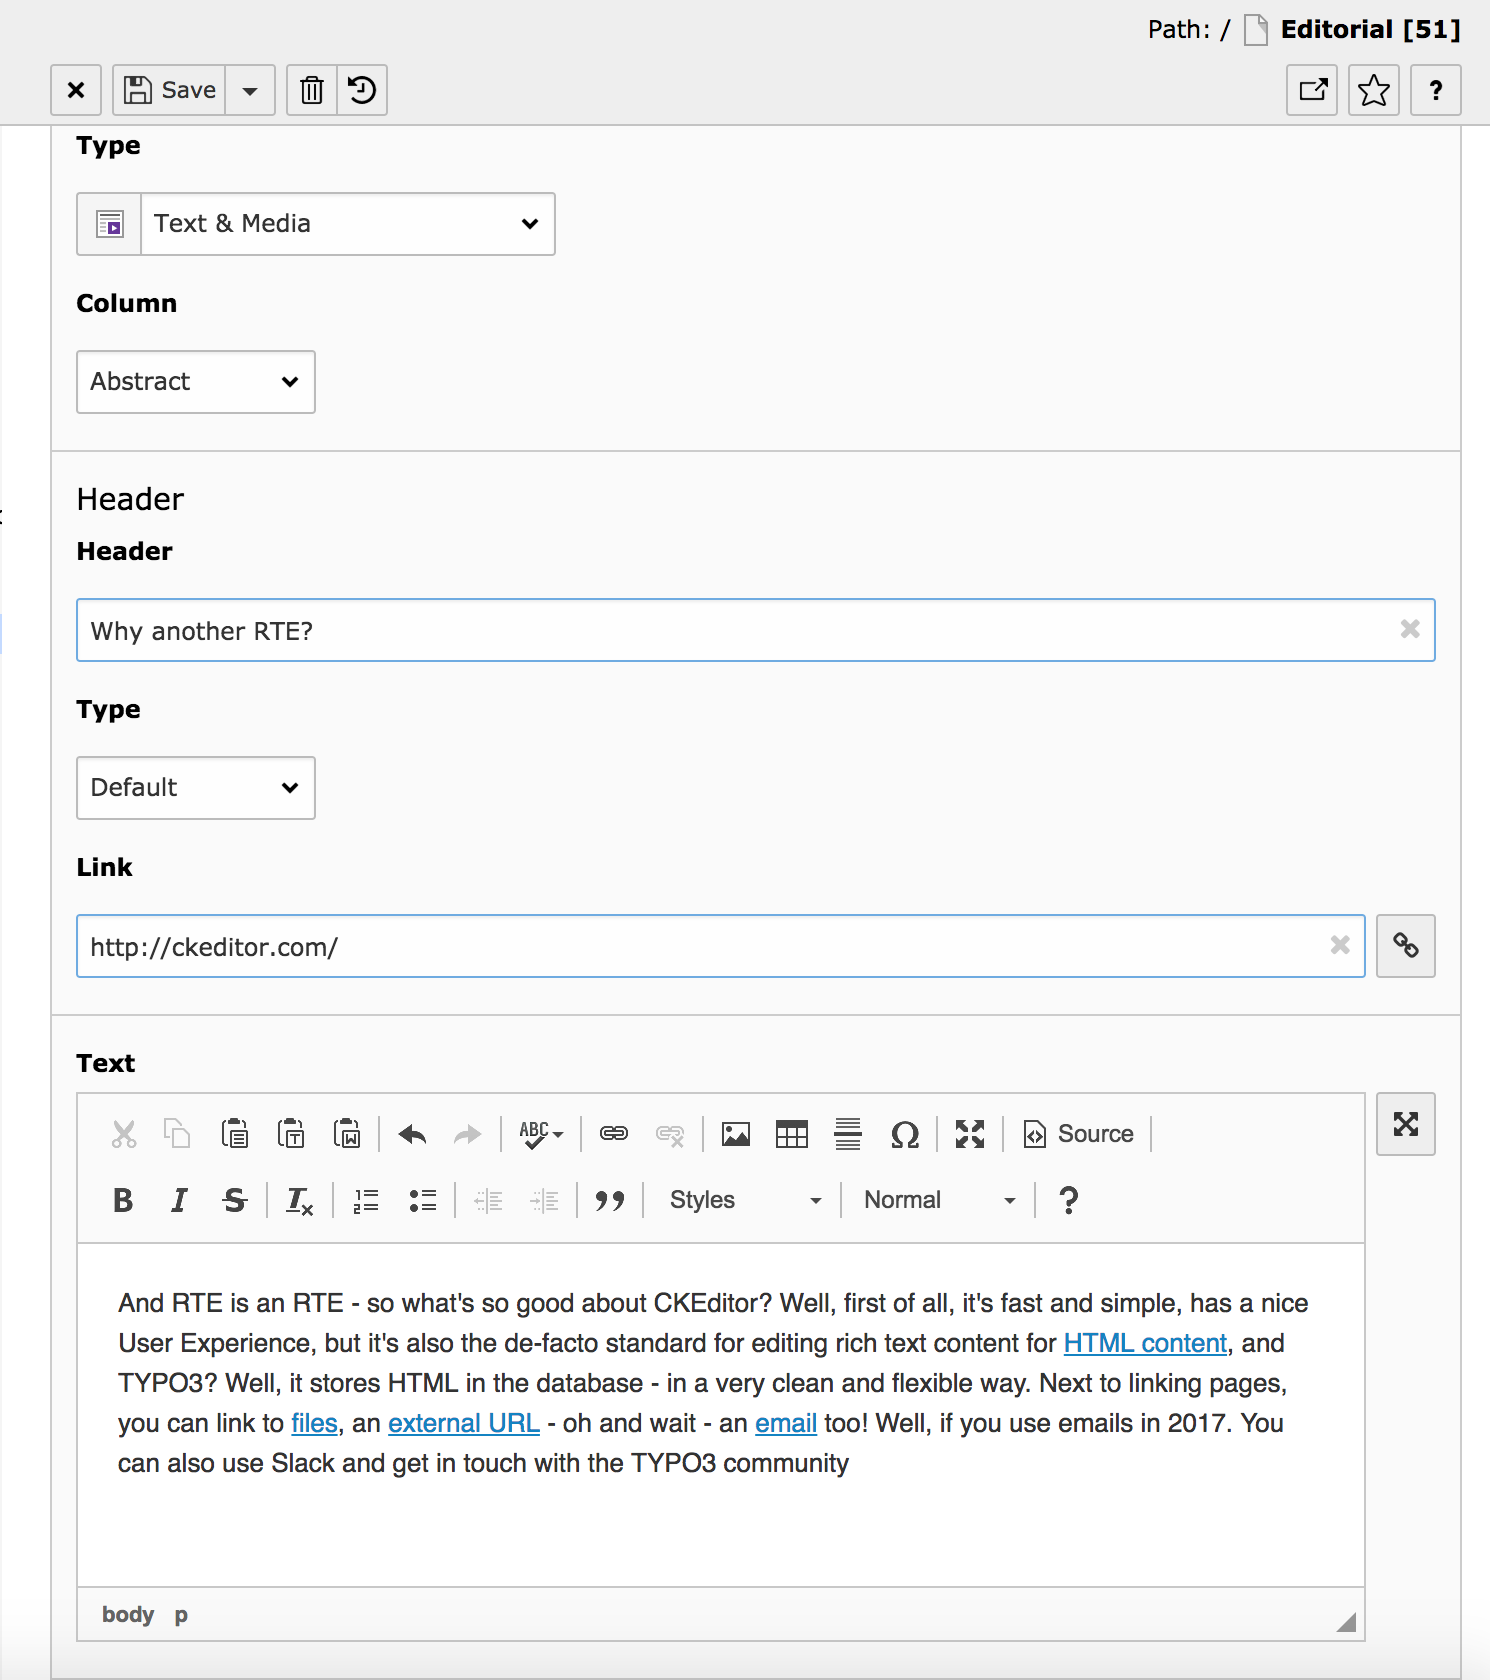
\includegraphics[width=0.8\linewidth]{BackendUserInterface/ckeditor.png}
			\end{figure}
		\end{column}
	\end{columns}

\end{frame}


% ------------------------------------------------------------------------------
% LTXE-SLIDE-START
% LTXE-SLIDE-UID:		6a41e672-ced4620b-ee3e255c-c9e1faba
% LTXE-SLIDE-ORIGIN:	c41b2f21-fb92bb80-56e7ddc9-1c725e34 English
% LTXE-SLIDE-TITLE:		CKEditor Integration
% ------------------------------------------------------------------------------
\begin{frame}[fragile]
	\frametitle{Interfaz de Usuario de Backend}
	\framesubtitle{Integración de CKEditor (2)}

	\begin{columns}[T]
		\begin{column}{.5\textwidth}
			Más detalles sobre este editor de código abierto: \url{http://ckeditor.com}
		\end{column}
		\begin{column}{.5\textwidth}
			\begin{figure}\vspace*{-0.4cm}
				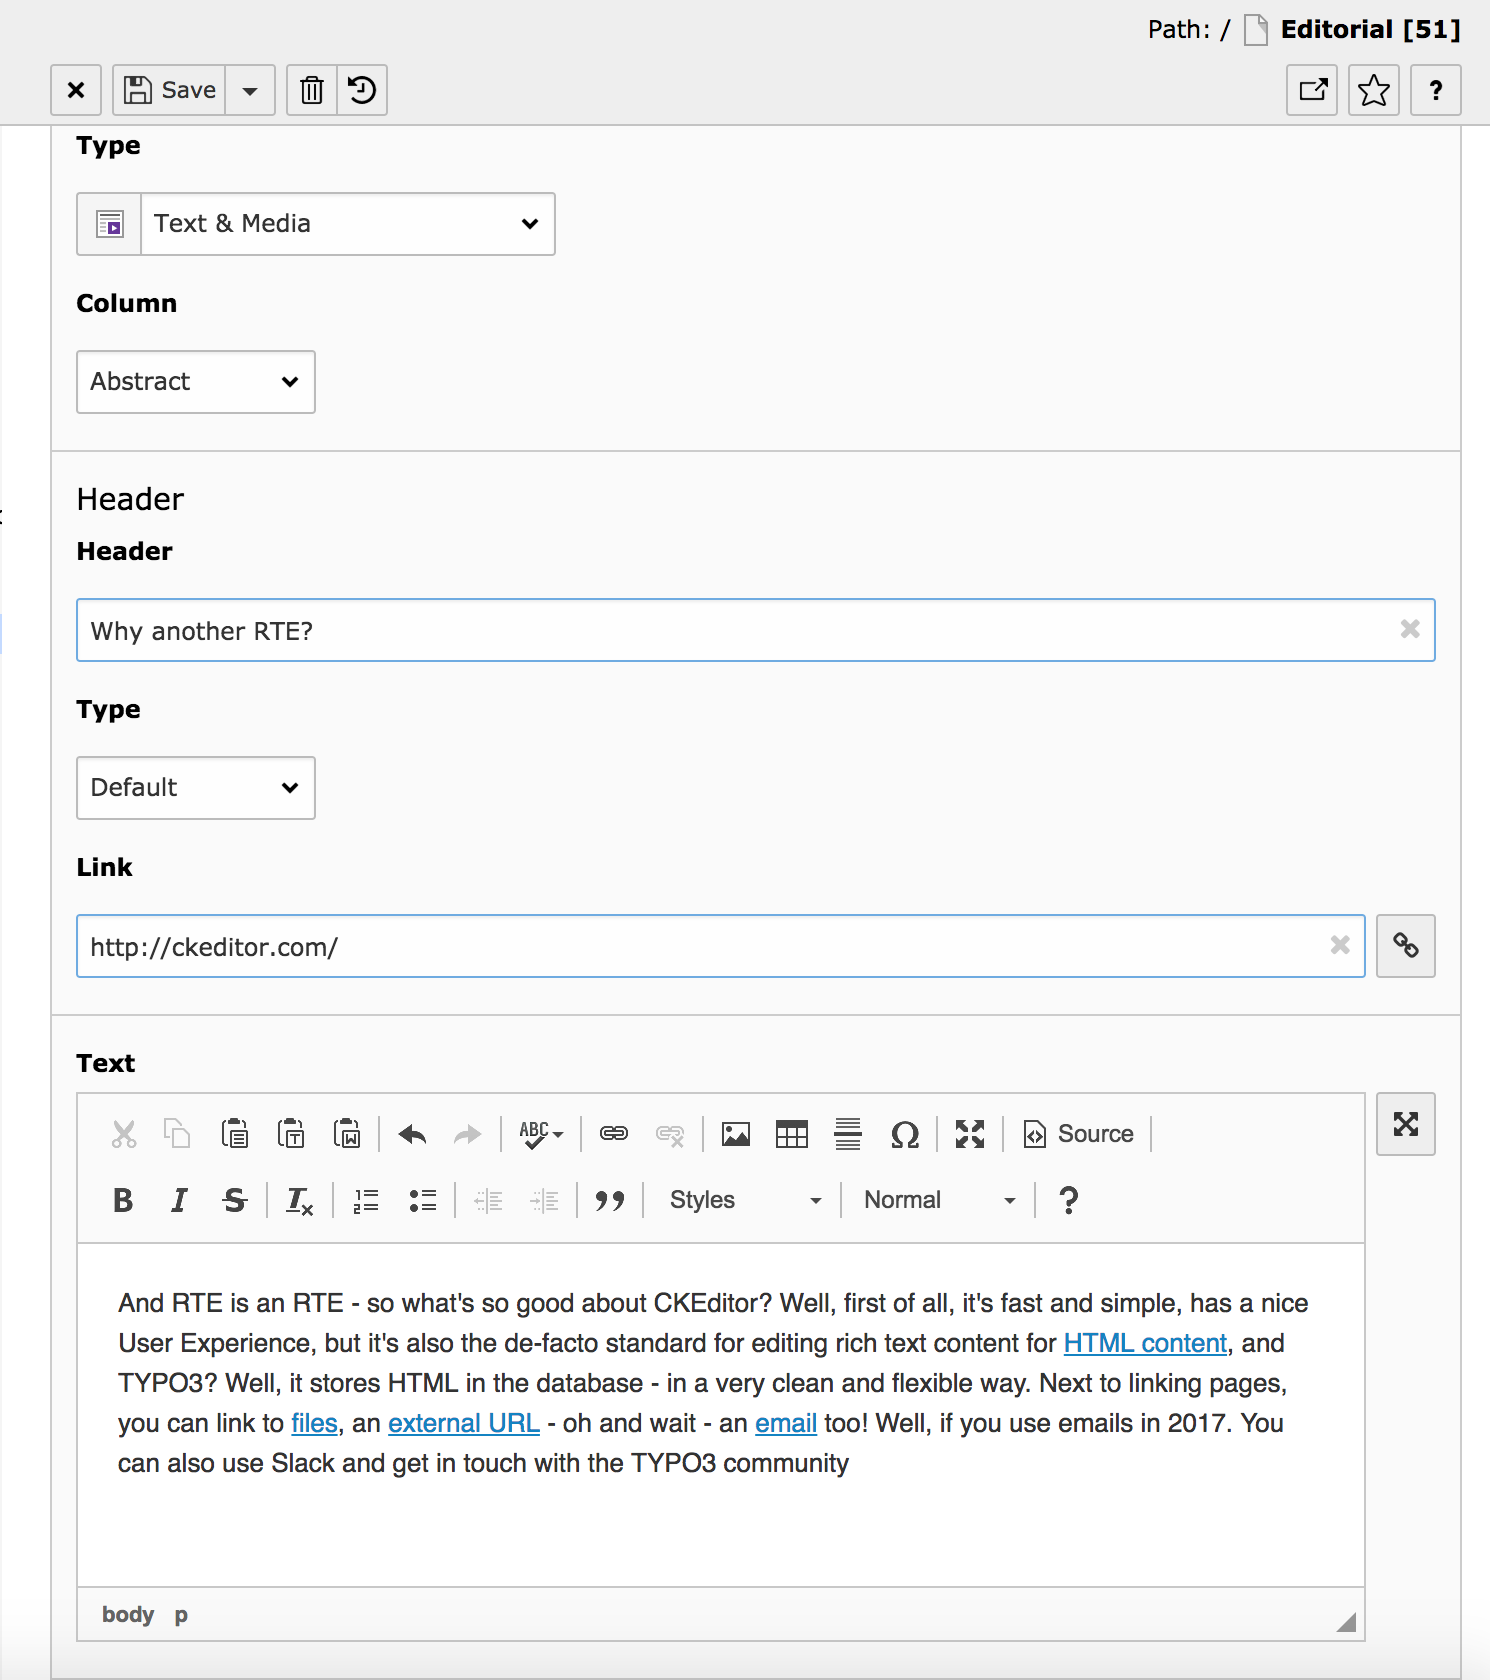
\includegraphics[width=0.8\linewidth]{BackendUserInterface/ckeditor.png}
			\end{figure}
		\end{column}
	\end{columns}

\end{frame}


% ------------------------------------------------------------------------------
% LTXE-SLIDE-START
% LTXE-SLIDE-UID:		f10b0914-85e50582-ecc561c7-90920367
% LTXE-SLIDE-ORIGIN:	c9dc360d-cf218f95-03f53731-03d821ad English
% LTXE-SLIDE-TITLE:		#78383: Field positions in tabs streamlined (TCA)
% ------------------------------------------------------------------------------
\begin{frame}[fragile]
	\frametitle{Interfaz de Usuario de Backend}
	\framesubtitle{Posición y Orden de Elementos}

	\begin{itemize}
		\item El orden y la posición de ciertos campos en el backend de TYPO3 ha sido dinamizada
		\item El propósito es cumplir la expectativa de los usuarios donde encontrar comonmente opciones usadas en la interfaz de usuario
		\item Esto es especialmente importante para recurrir a definiciones de campo y categorías genéricas compartidas por un montón de registros
		\item Se anima a los autores de extensiones a seguir las posiciones y órdenes de elementos especificados en
			la \href{https://docs.typo3.org}{documentación oficial}

			% TODO: update link above (waiting for Doc and Core Team to finish documentation)

	\end{itemize}

	\begin{itemize}
		\item \textit{La consistencia del backend es lo que manda!} :-)
	\end{itemize}

\end{frame}

% ------------------------------------------------------------------------------
